\documentclass{article}
\usepackage[margin=1in]{geometry}
\usepackage[utf8]{inputenc}
\usepackage{amsfonts,amsmath,bm}
\usepackage{xcolor}
\usepackage{graphicx}
\usepackage{caption}
\usepackage{subcaption}
\usepackage{tabulary}
\usepackage{multirow}
\usepackage{algorithm}
\usepackage{algpseudocode}
% \usepackage{biblatex}
% \addbibresource{bibliography.bib} %Import the bibliography file
% \usepackage[framed,numbered,autolinebreaks,useliterate]{mcode}
\usepackage{tikz}
\newcommand*\circled[1]{\tikz[baseline= (char.base)]{
            \node[shape=circle, draw, inner sep=1.5pt] (char) {#1};}}
\newcommand*\smallcircled[1]{\tikz[baseline= (char.base)]{
            \node[shape=circle, draw, inner sep=0.5pt] (char) {#1};}}


\title{EEC269A - Error Correcting Codes I\\Project Report}
\author{Chenye Yang, Pranav Kharche, Parisa Oftadeh}
\date{\today}

\begin{document}

\maketitle

\section{Workload}


\begin{center}
    \renewcommand{\arraystretch}{1.5}
    \begin{tabulary}{\textwidth}{ |L|L|L| } 
    \hline
    \textbf{Function} & \textbf{Workload} & \textbf{Contributor} \\
    \hline
    Source & Text string (TXT), Image (PNG), Audio (WAV) & Chenye \\ 
    \hline
    \multirow{2}{*}{Encoder} & $(7,4)$ Systematic Linear Block (Hamming) Code & Chenye \\ 
    & $(n,k)$ Systematic Cyclic (Hamming) Code & Pranav, Chenye \\ 
    \hline
    \multirow{1}{*}{Channel} & Binary Symmetric Channel (BSC), error probability $p$ adjustable & Chenye \\ 
    \hline
    \multirow{3}{*}{Error Corrector} &  Syndrome Lookup Table for $(7,4)$ Linear Code & Chenye \\ 
    & Syndrome Lookup Table for $(n,k)$ Cyclic Code & Chenye \\ 
    & LFSR for $(n,k)$ Cyclic Code & \textcolor{red}{TODO} \\
    \hline
    \multirow{2}{*}{Decoder} & $(7,4)$ Systematic Linear Block (Hamming) Code & Chenye \\ 
    & $(n,k)$ Systematic Cyclic (Hamming) Code & Chenye \\ 
    \hline
    Destination & Text string (TXT), Image (PNG), Audio (WAV) & Chenye \\ 
    \hline
    \multirow{2}{*}{\textbf{Advanced}} & \textbf{Create generator matrix for $(n,k)$ cyclic code} & Pranav \\ 
    & \textbf{Adjustable $(n,k)$} & Pranav \\ 
    \hline
    \end{tabulary}
\end{center}


\section{(7,4) Systematic Linear Block (Hamming) Code}
\subsection{Syndrome Decoder}
\subsubsection{Text string}

\begin{center}
    \renewcommand{\arraystretch}{1.5}
    \begin{tabulary}{\textwidth}{ |L|L|L| } 
    \hline
    \textbf{Original} & \textbf{Without correction} & \textbf{Corrected} \\
    \hline
    Hello World! EEC269A Error Correcting Code Demo & Hello Wo\textcolor{red}{p}ld! EEC269A \textcolor{red}{A}rror Correcting \textcolor{red}{K}ode Demo & Hello World! EEC269A Error Correcting Code Demo \\
    \hline
    \end{tabulary}
\end{center}



\subsubsection{Image}


\begin{figure}
    \centering
    \begin{subfigure}[b]{0.32\textwidth}
        \centering
        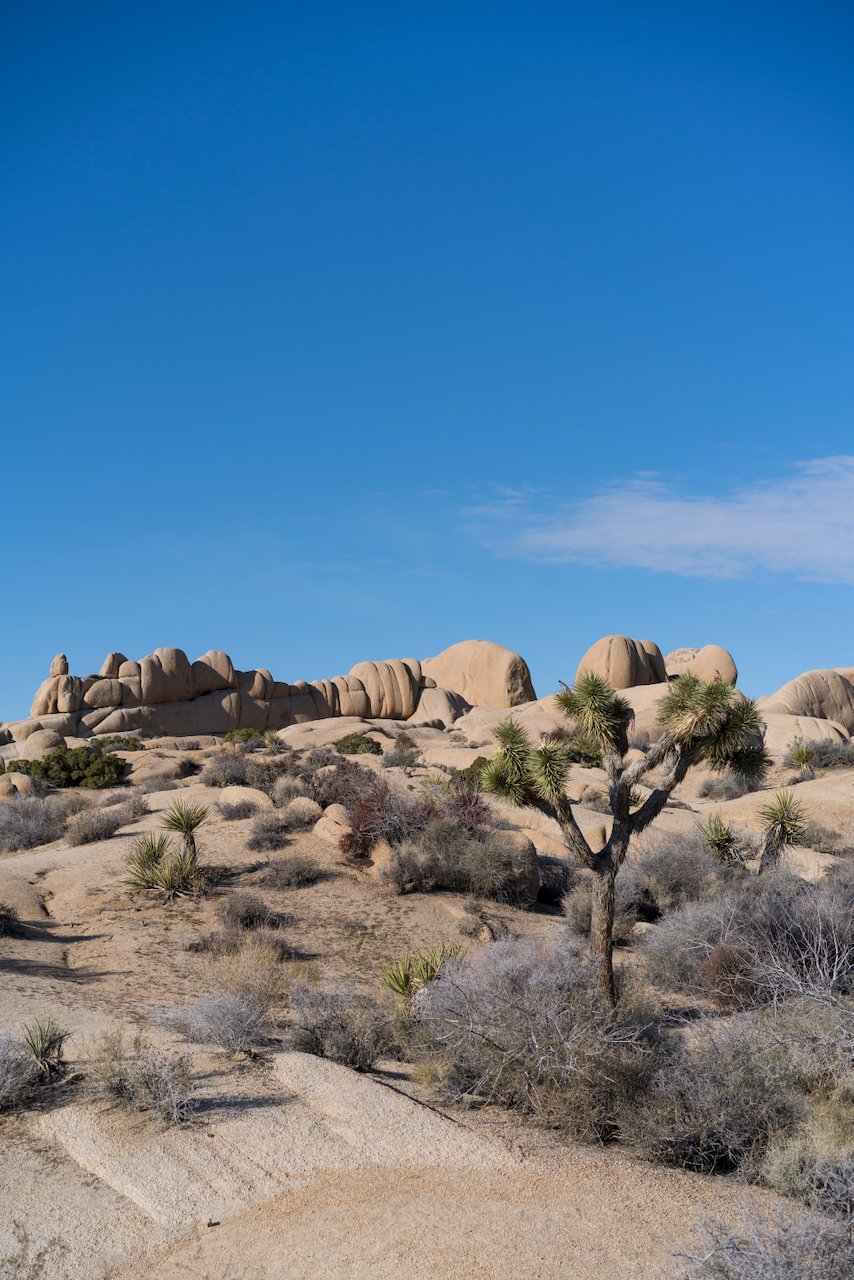
\includegraphics[width=\textwidth]{../Resource/image.png}
        \caption{Original}
        \label{fig:image-linear-bsc-original}
    \end{subfigure}
    \hfill
    \begin{subfigure}[b]{0.32\textwidth}
        \centering
        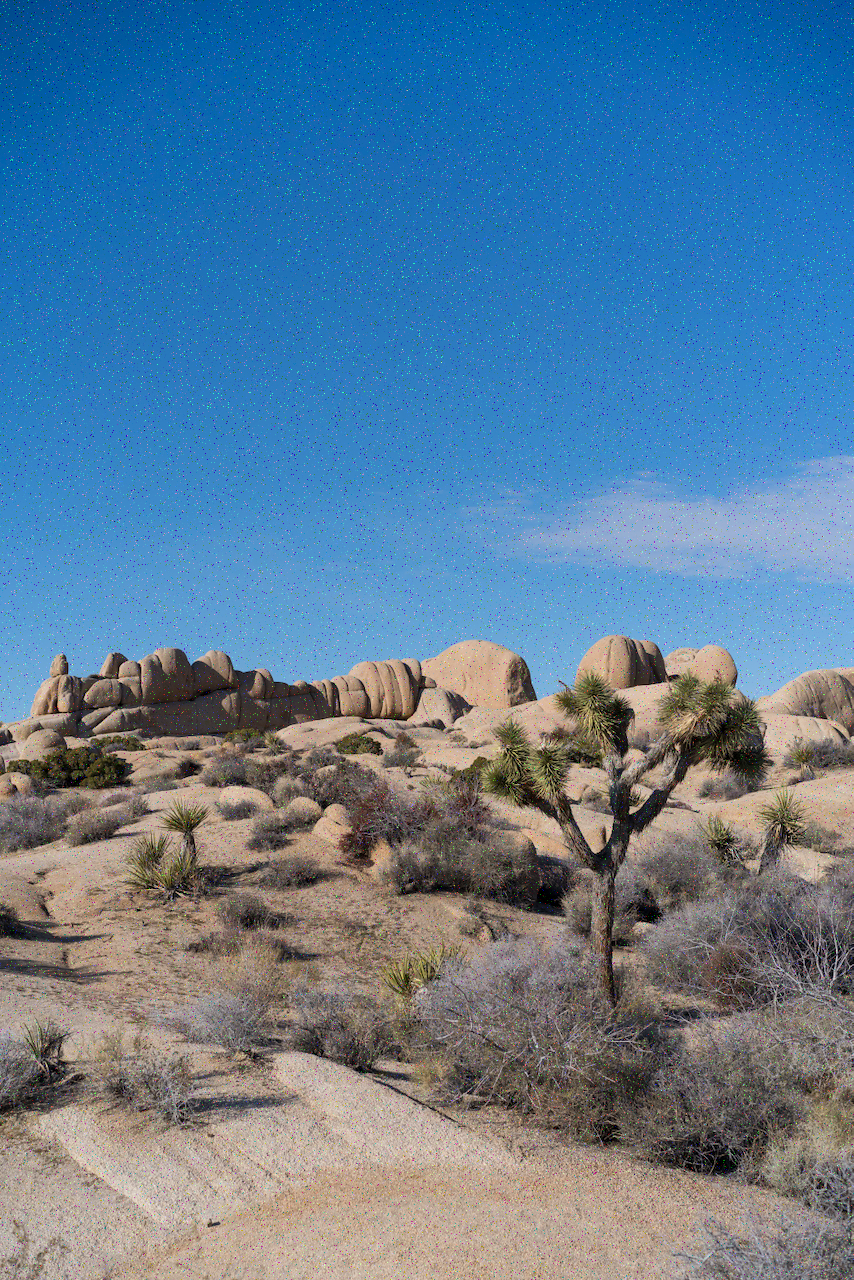
\includegraphics[width=\textwidth]{../Result/linear-bsc-output.png}
        \caption{Without correction}
        \label{fig:image-linear-bsc-no-correction}
    \end{subfigure}
    \hfill
    \begin{subfigure}[b]{0.32\textwidth}
        \centering
        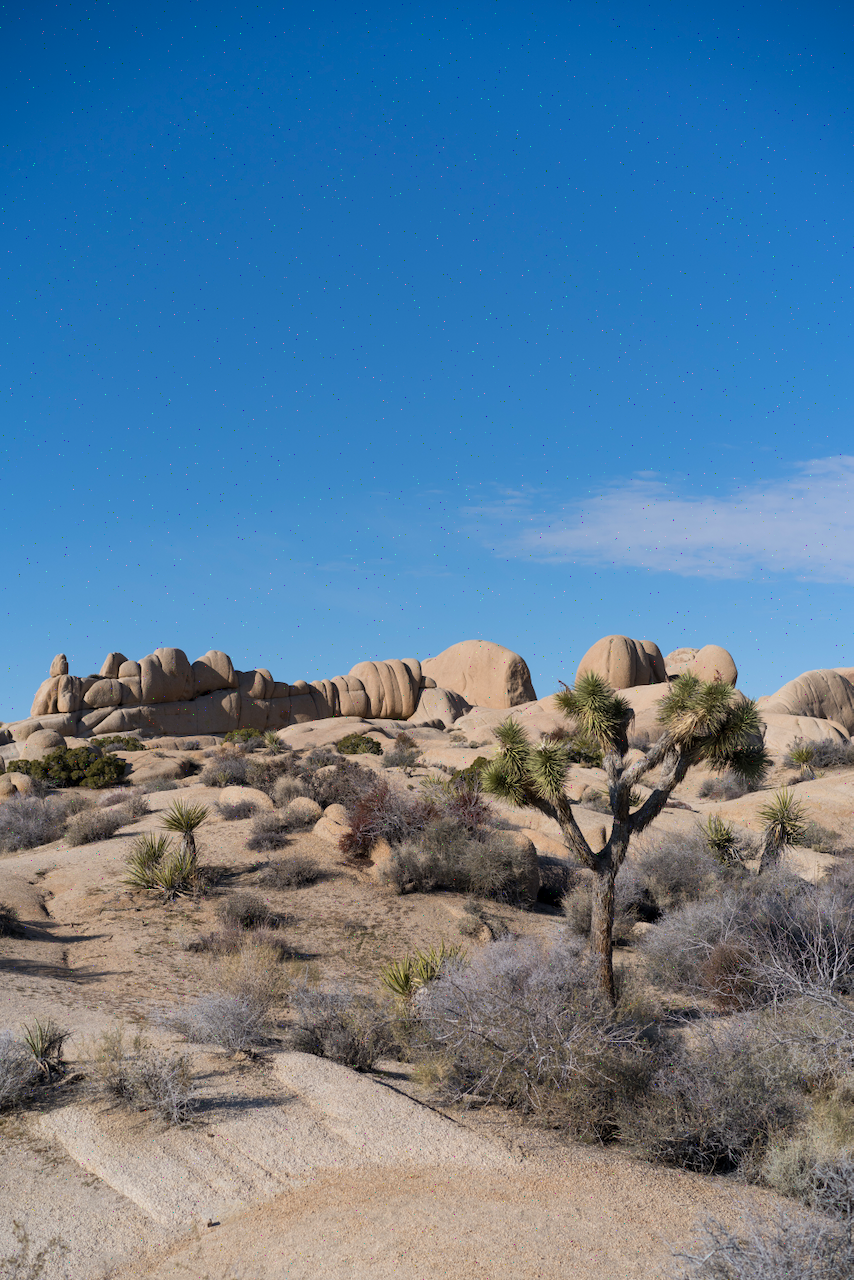
\includegraphics[width=\textwidth]{../Result/linear-bsc-output-syndrome-corrected.png}
        \caption{Corrected}
        \label{fig:image-linear-bsc-syndrome-corrected}
    \end{subfigure}
       \caption{Image encoded with Linear Hamming passed through BSC (entire)}
       \label{fig:image-linear-bsc}
\end{figure}


\begin{figure}
    \centering
    \begin{subfigure}[b]{0.32\textwidth}
        \centering
        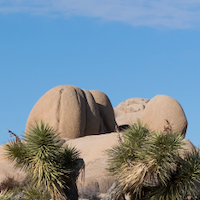
\includegraphics[width=\textwidth]{../Resource/cropped-image.png}
        \caption{Original}
        \label{fig:cropped-image-linear-bsc-original}
    \end{subfigure}
    \hfill
    \begin{subfigure}[b]{0.32\textwidth}
        \centering
        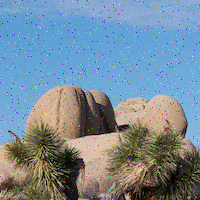
\includegraphics[width=\textwidth]{../Result/cropped-linear-bsc-output.png}
        \caption{Without correction}
        \label{fig:cropped-image-linear-bsc-no-correction}
    \end{subfigure}
    \hfill
    \begin{subfigure}[b]{0.32\textwidth}
        \centering
        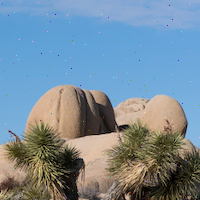
\includegraphics[width=\textwidth]{../Result/cropped-linear-bsc-output-syndrome-corrected.png}
        \caption{Corrected}
        \label{fig:cropped-image-linear-bsc-syndrome-corrected}
    \end{subfigure}
       \caption{Image encoded with Linear Hamming passed through BSC (details)}
       \label{fig:cropped-image-linear-bsc}
\end{figure}


\subsubsection{Audio}


\begin{figure}
    \centering
    \begin{subfigure}[b]{\textwidth}
        \centering
        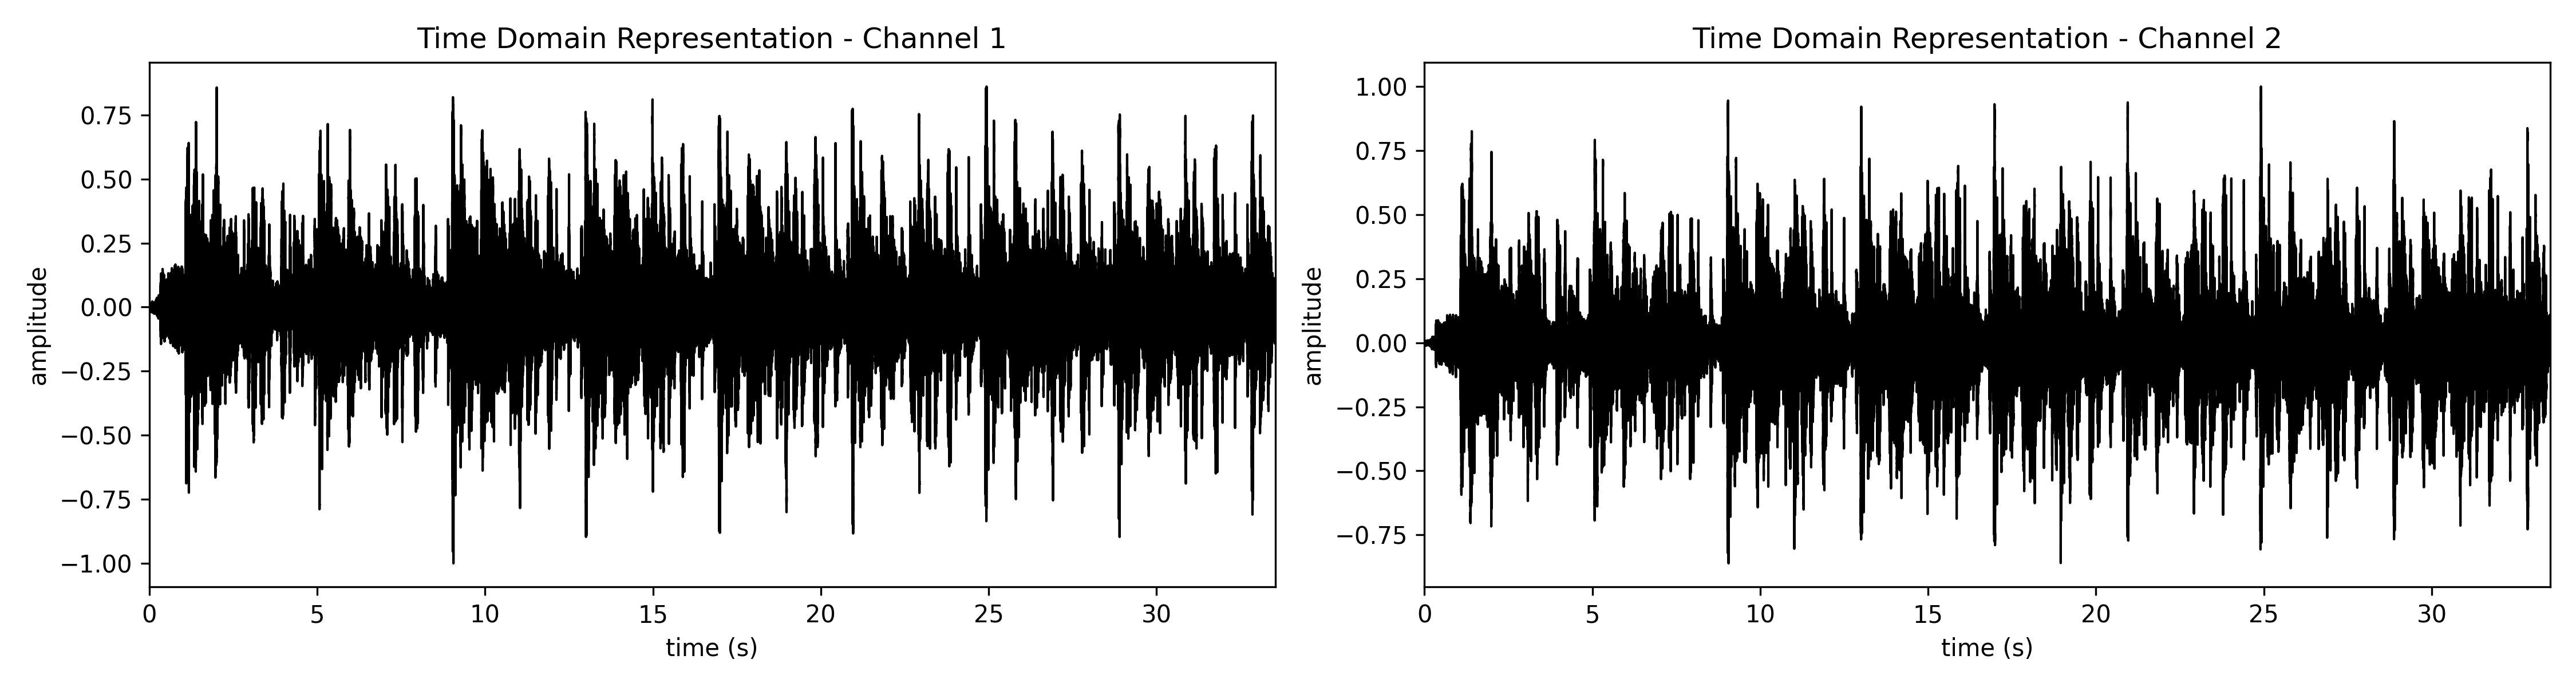
\includegraphics[width=\textwidth]{../Result/wav-time-domain-TX.png}
        \caption{Original}
        \label{fig:t-audio-linear-bsc-original}
    \end{subfigure}
    % \hfill
    \begin{subfigure}[b]{\textwidth}
        \centering
        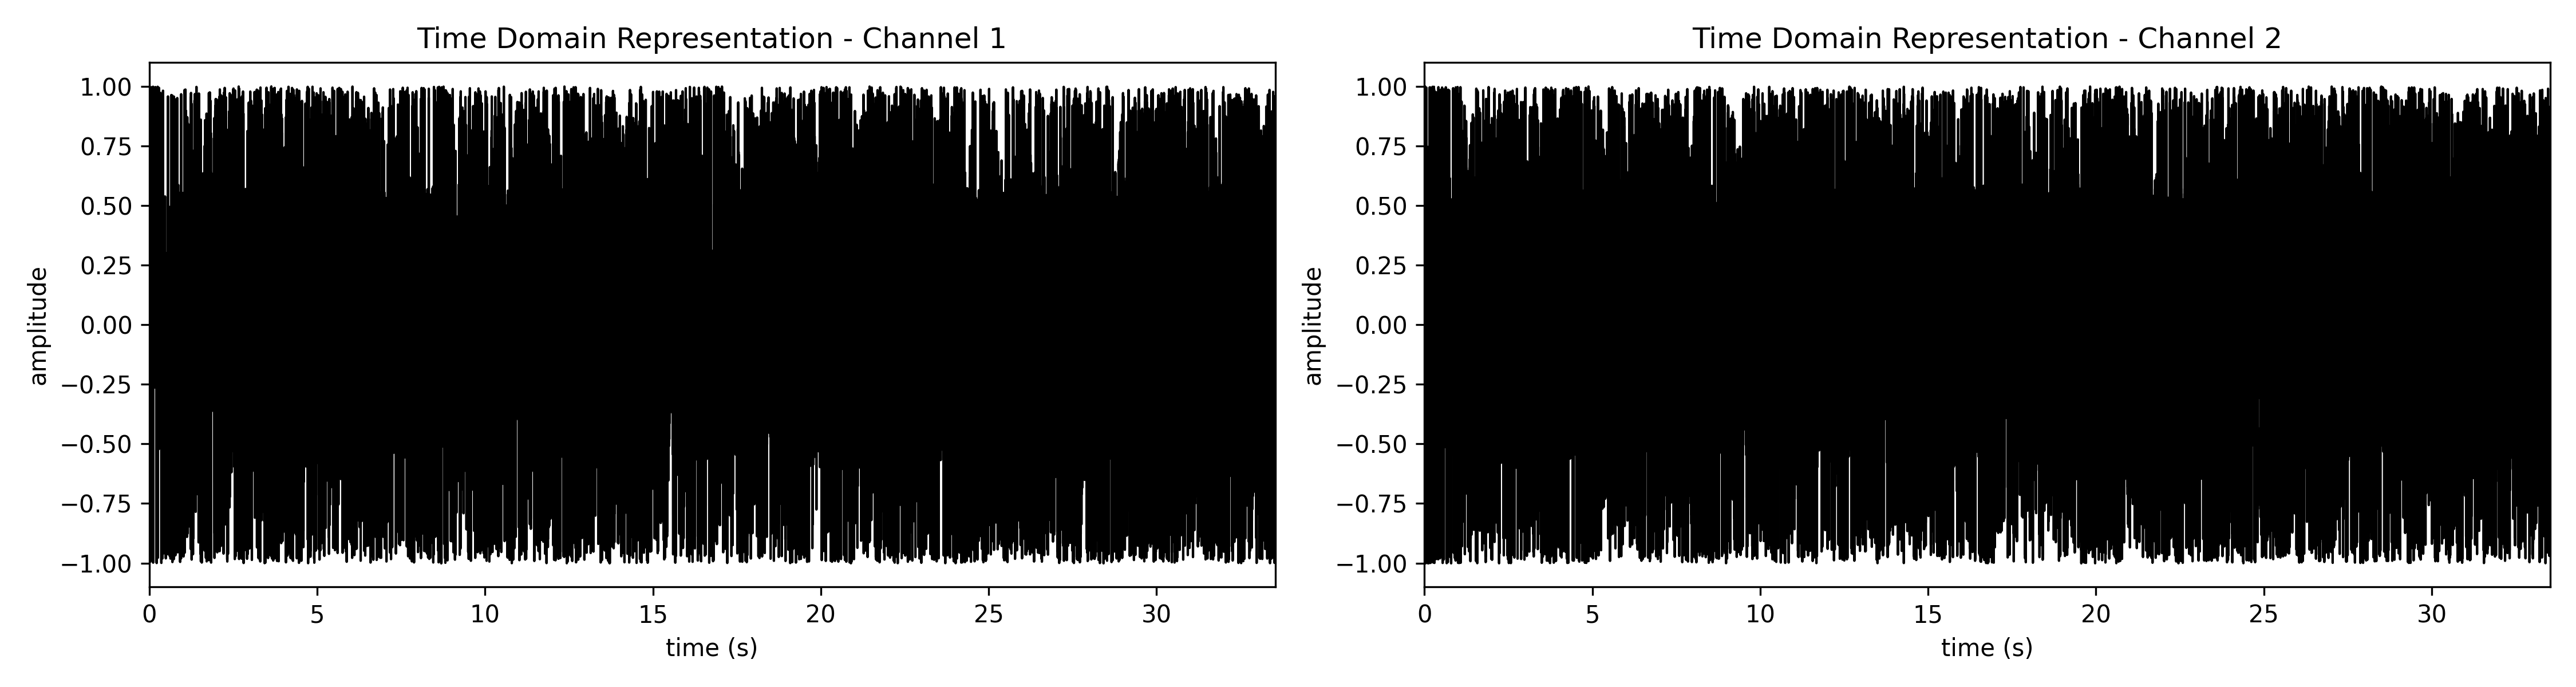
\includegraphics[width=\textwidth]{../Result/linear-bsc-wav-time-domain-RX.png}
        \caption{Without correction}
        \label{fig:t-audio-linear-bsc-no-correction}
    \end{subfigure}
    % \hfill
    \begin{subfigure}[b]{\textwidth}
        \centering
        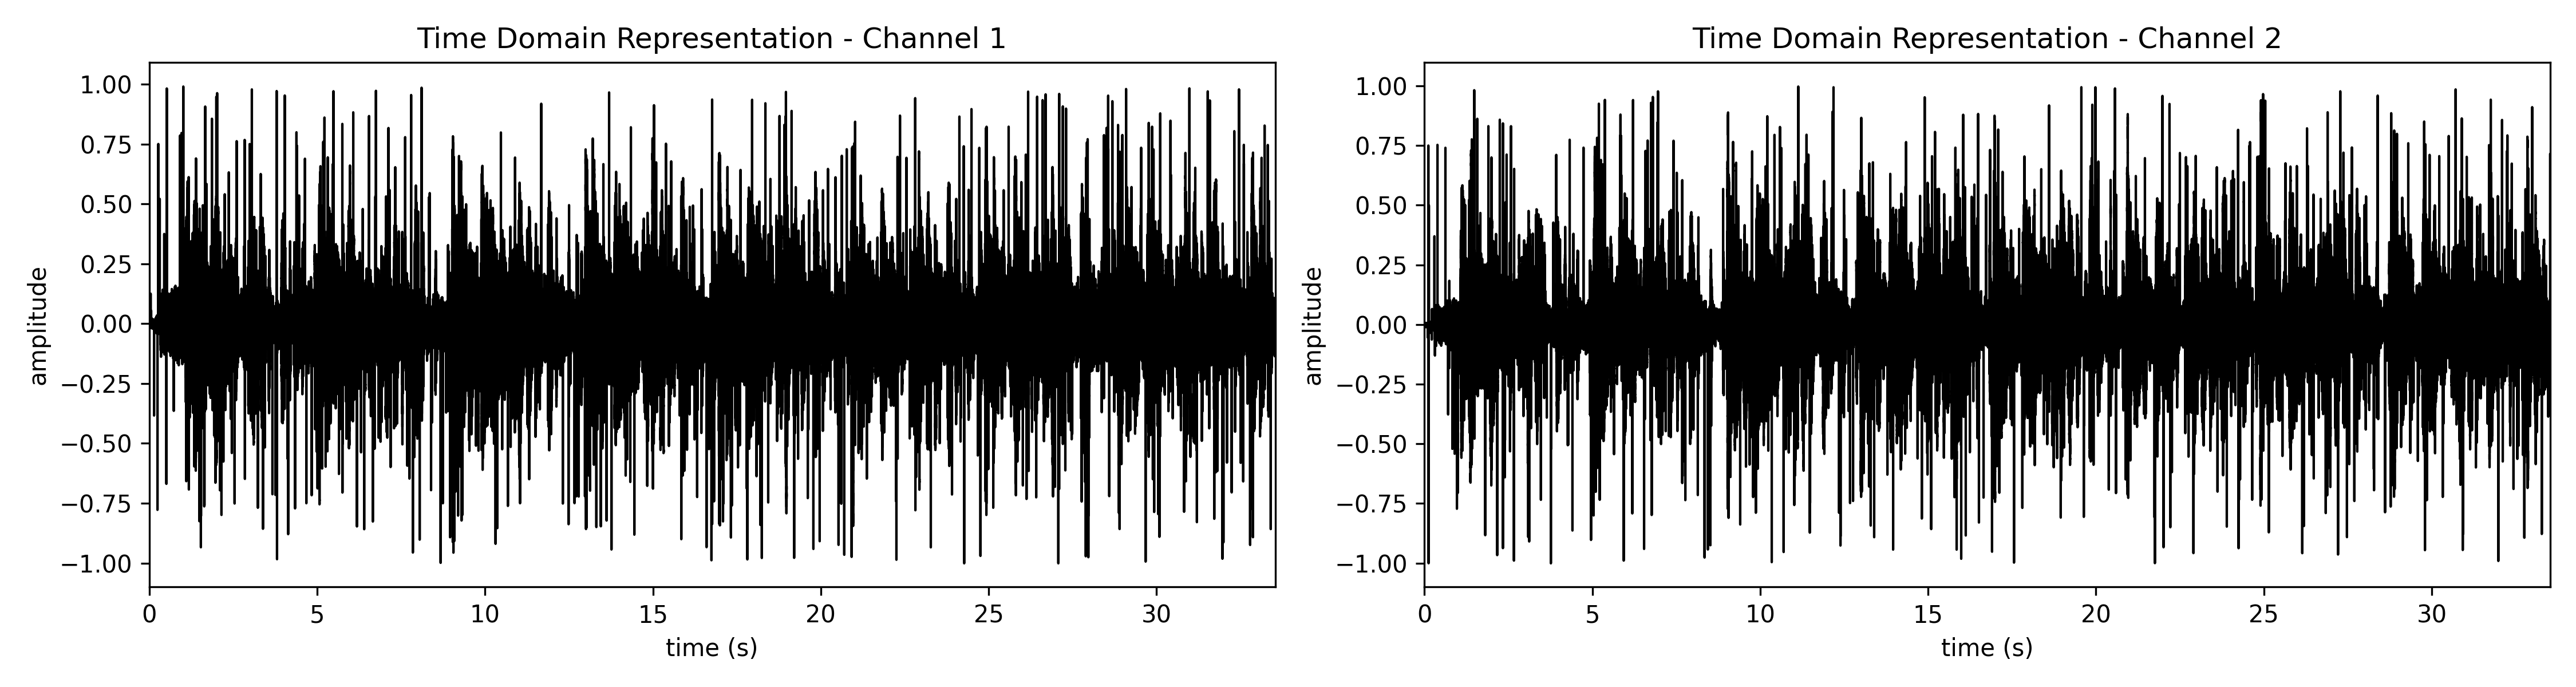
\includegraphics[width=\textwidth]{../Result/linear-bsc-wav-time-domain-RX-syndrome-corrected.png}
        \caption{Corrected}
        \label{fig:t-audio-linear-bsc-syndrome-syndrome-corrected}
    \end{subfigure}
       \caption{Audio encoded with Linear Hamming passed through BSC}
       \label{fig:t-audio-linear-bsc}
\end{figure}


\begin{figure}
    \centering
    \begin{subfigure}[b]{\textwidth}
        \centering
        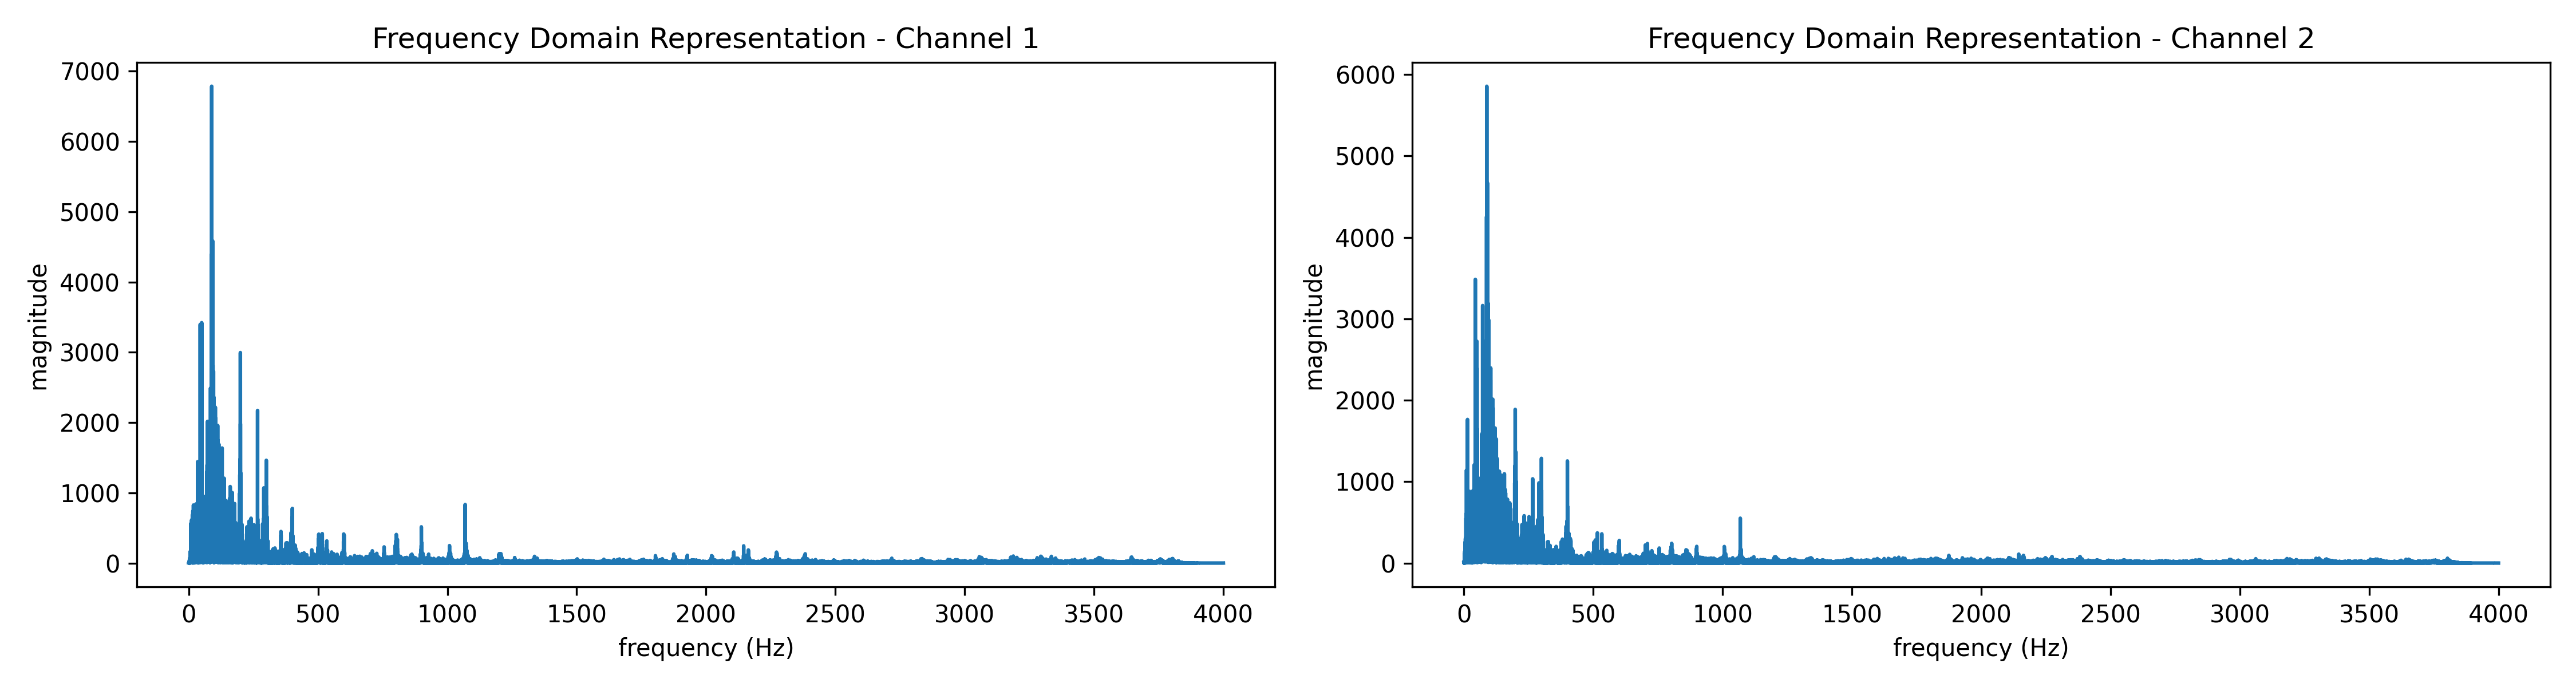
\includegraphics[width=\textwidth]{../Result/wav-frequency-domain-TX.png}
        \caption{Original}
        \label{fig:f-audio-linear-bsc-original}
    \end{subfigure}
    % \hfill
    \begin{subfigure}[b]{\textwidth}
        \centering
        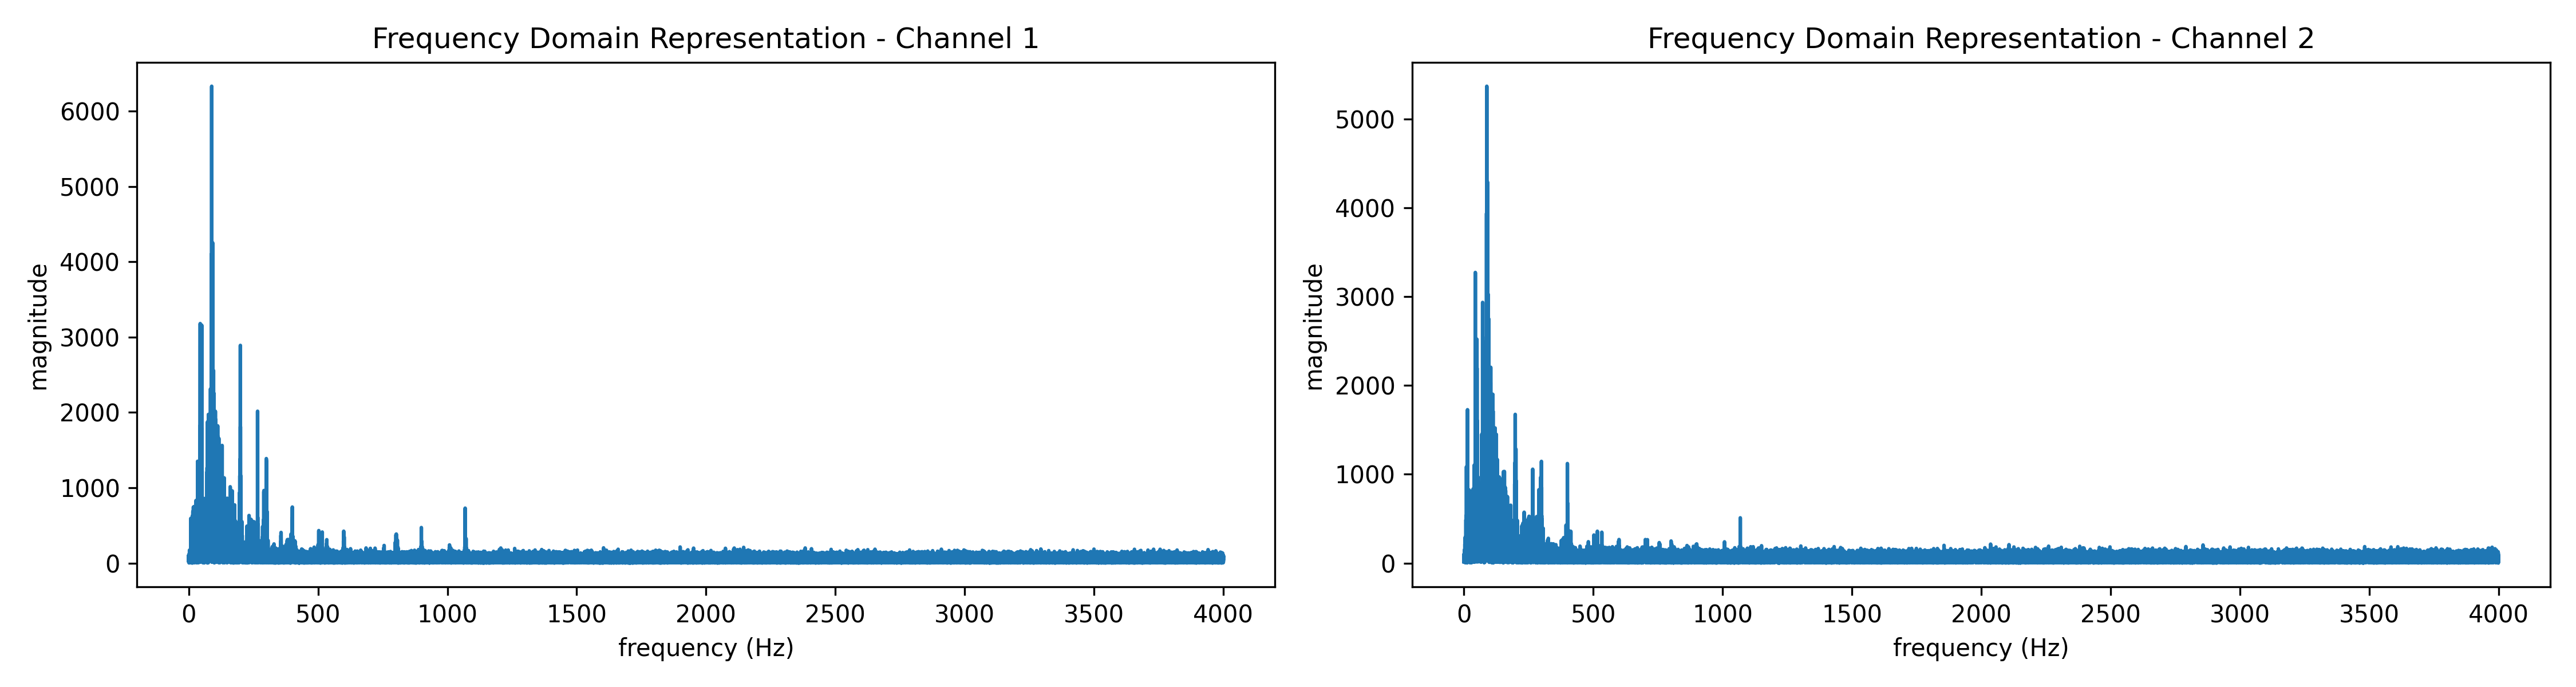
\includegraphics[width=\textwidth]{../Result/linear-bsc-wav-frequency-domain-RX.png}
        \caption{Without correction}
        \label{fig:f-audio-linear-bsc-no-correction}
    \end{subfigure}
    % \hfill
    \begin{subfigure}[b]{\textwidth}
        \centering
        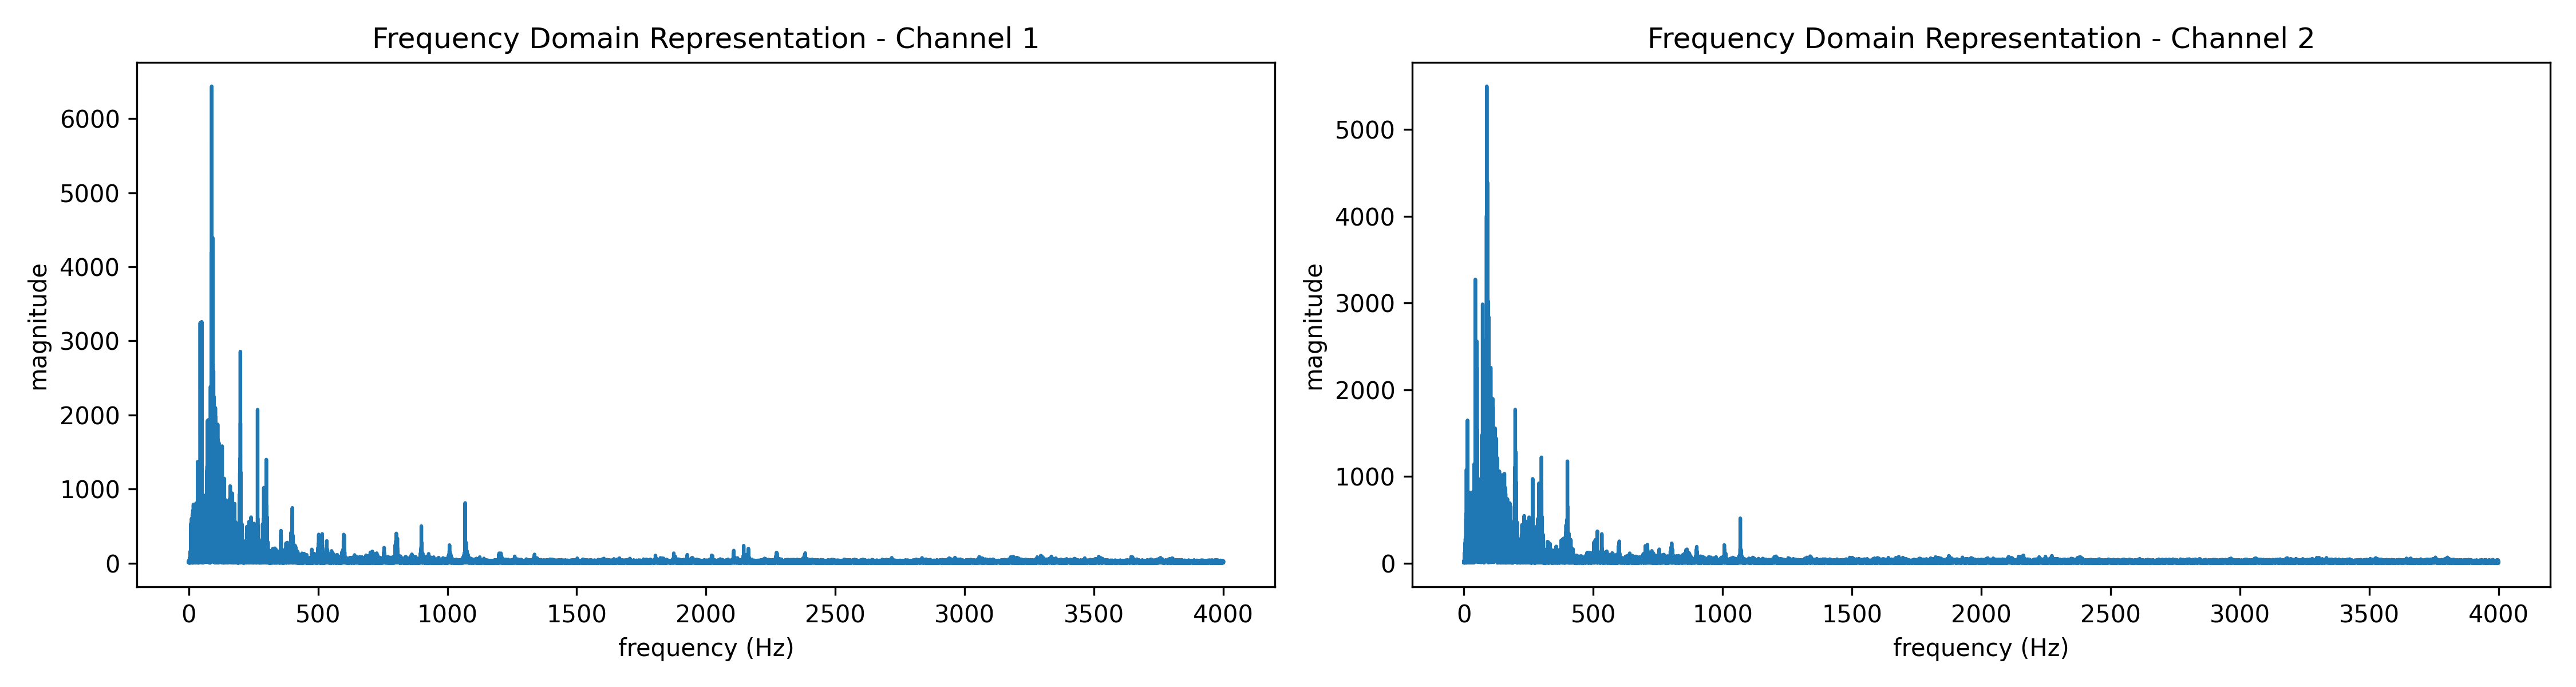
\includegraphics[width=\textwidth]{../Result/linear-bsc-wav-frequency-domain-RX-syndrome-corrected.png}
        \caption{Corrected}
        \label{fig:f-audio-linear-bsc-syndrome-corrected}
    \end{subfigure}
       \caption{Audio encoded with Linear Hamming passed through BSC}
       \label{fig:f-audio-linear-bsc}
\end{figure}


\section{$(n,k)$ Systematic Cyclic (Hamming) Code}
\subsection{Syndrome Decoder}
\subsubsection{Text string}


\begin{center}
    \renewcommand{\arraystretch}{1.5}
    \begin{tabulary}{\textwidth}{ |L|L|L| } 
    \hline
    \textbf{Original} & \textbf{Without correction} & \textbf{Corrected} \\
    \hline
    Hello World! EEC269A Error Correcting Code Demo & H\textcolor{red}{u,}lo World! EEC269A Error Correcti\textcolor{red}{f}g Code Demo & Hello World! EEC269A Error Correcting Code Demo \\
    \hline
    \end{tabulary}
\end{center}



\subsubsection{Image}


\begin{figure}
    \centering
    \begin{subfigure}[b]{0.32\textwidth}
        \centering
        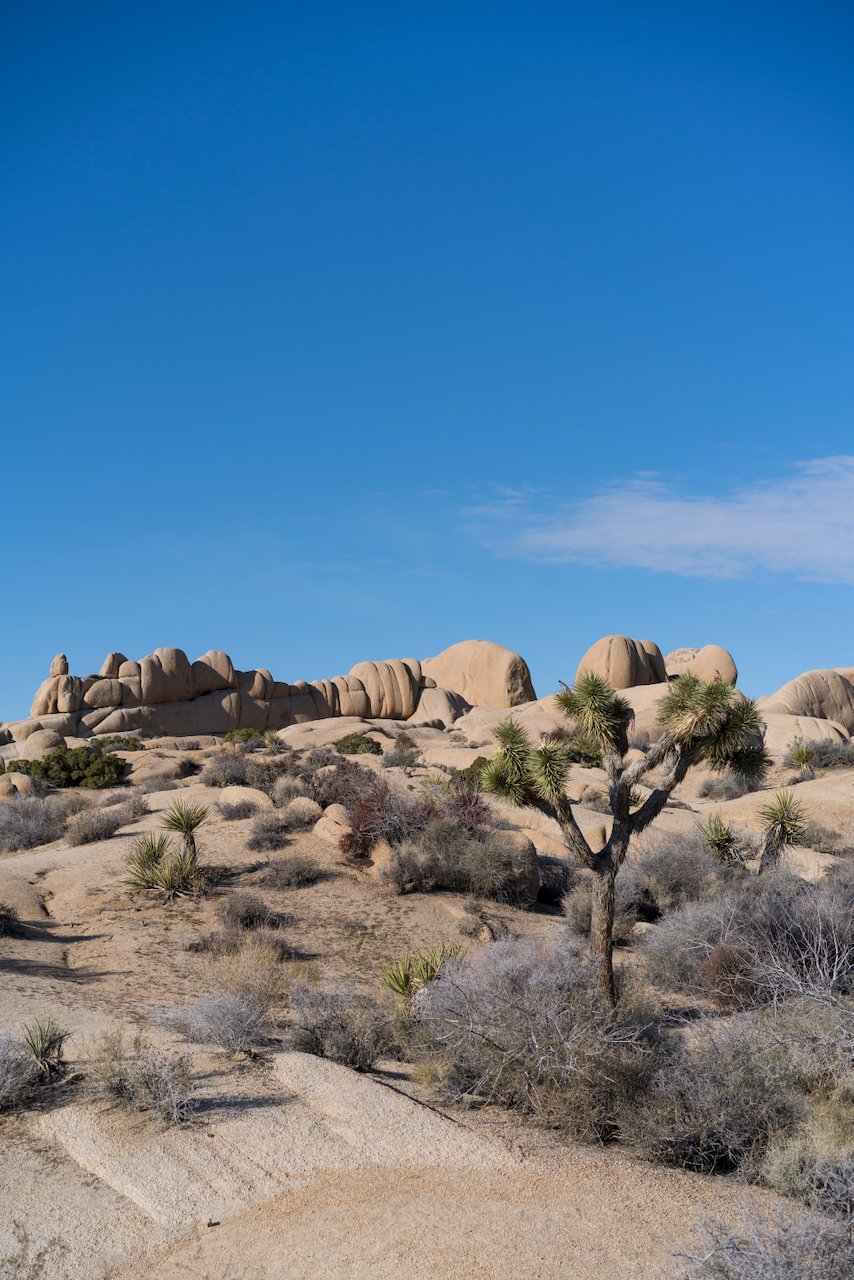
\includegraphics[width=\textwidth]{../Resource/image.png}
        \caption{Original}
        \label{fig:image-cyclic-bsc-original}
    \end{subfigure}
    \hfill
    \begin{subfigure}[b]{0.32\textwidth}
        \centering
        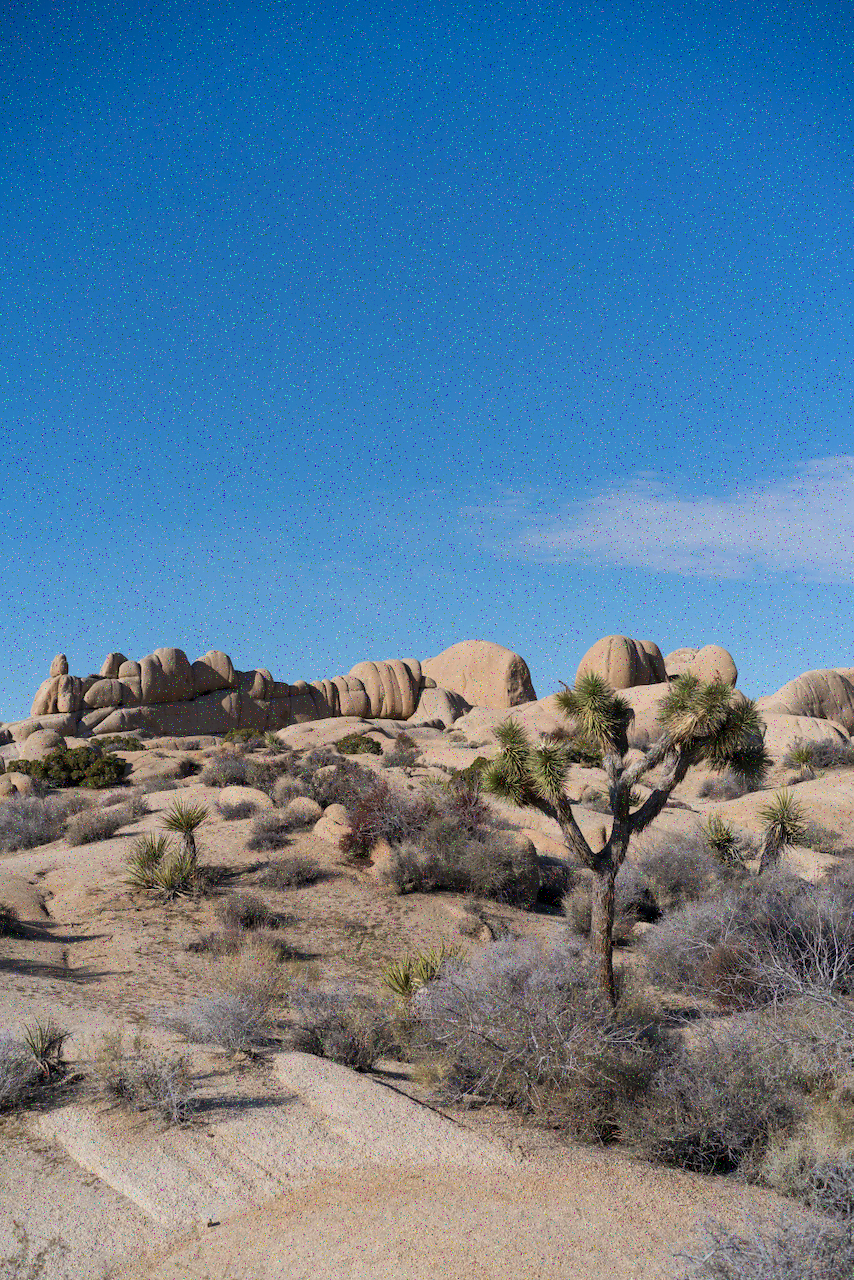
\includegraphics[width=\textwidth]{../Result/cyclic-bsc-output.png}
        \caption{Without correction}
        \label{fig:image-cyclic-bsc-no-correction}
    \end{subfigure}
    \hfill
    \begin{subfigure}[b]{0.32\textwidth}
        \centering
        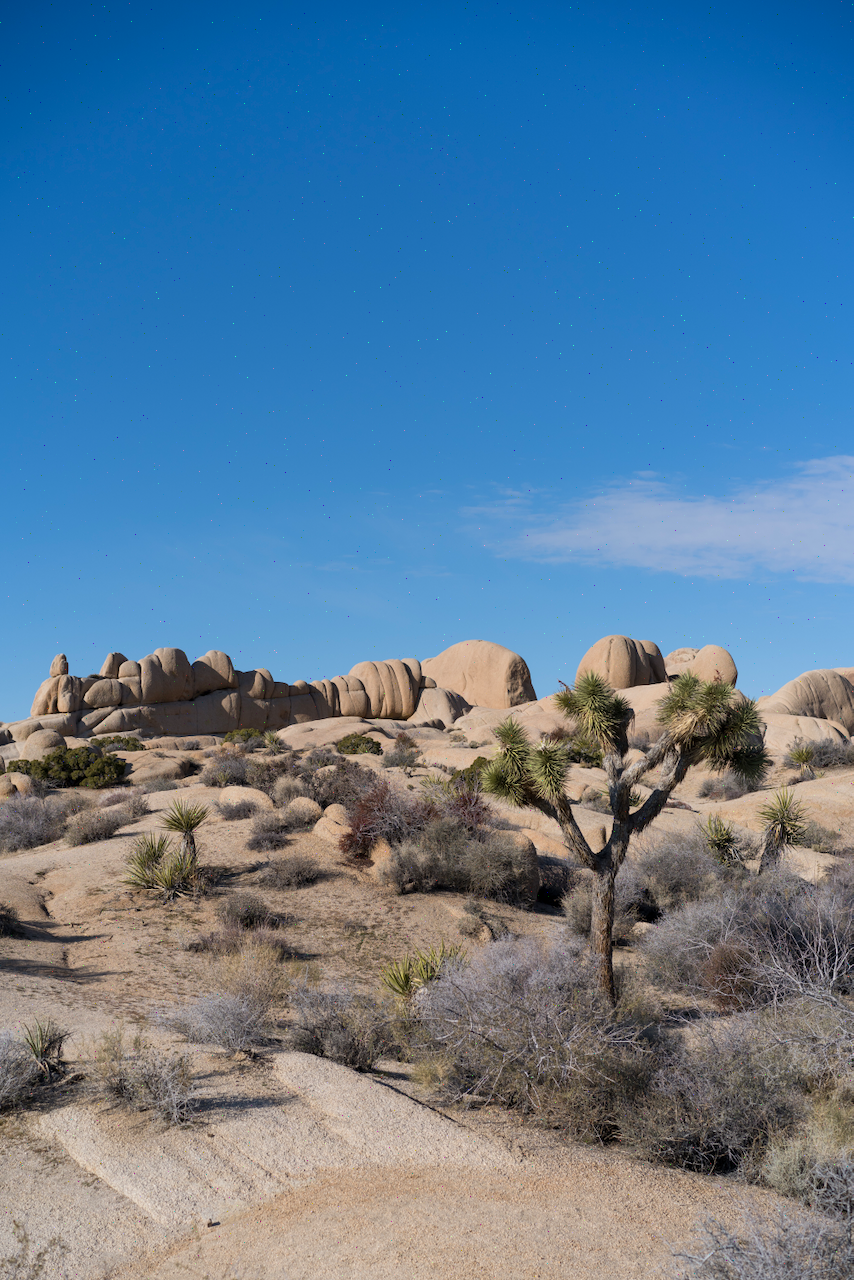
\includegraphics[width=\textwidth]{../Result/cyclic-bsc-output-syndrome-corrected.png}
        \caption{Corrected}
        \label{fig:image-cyclic-bsc-syndrome-corrected}
    \end{subfigure}
       \caption{Image encoded with Cyclic Hamming passed through BSC (entire)}
       \label{fig:image-cyclic-bsc}
\end{figure}




\begin{figure}
    \centering
    \begin{subfigure}[b]{0.32\textwidth}
        \centering
        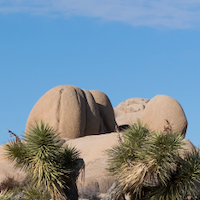
\includegraphics[width=\textwidth]{../Resource/cropped-image.png}
        \caption{Original}
        \label{fig:cropped-image-cyclic-bsc-original}
    \end{subfigure}
    \hfill
    \begin{subfigure}[b]{0.32\textwidth}
        \centering
        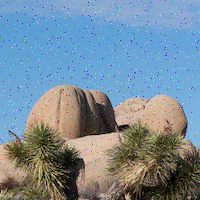
\includegraphics[width=\textwidth]{../Result/cropped-cyclic-bsc-output.png}
        \caption{Without correction}
        \label{fig:cropped-image-cyclic-bsc-no-correction}
    \end{subfigure}
    \hfill
    \begin{subfigure}[b]{0.32\textwidth}
        \centering
        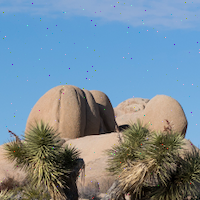
\includegraphics[width=\textwidth]{../Result/cropped-cyclic-bsc-output-syndrome-corrected.png}
        \caption{Corrected}
        \label{fig:cropped-image-cyclic-bsc-syndrome-corrected}
    \end{subfigure}
       \caption{Image encoded with Cyclic Hamming passed through BSC (details)}
       \label{fig:cropped-image-cyclic-bsc}
\end{figure}






\subsubsection{Audio}



\begin{figure}
    \centering
    \begin{subfigure}[b]{\textwidth}
        \centering
        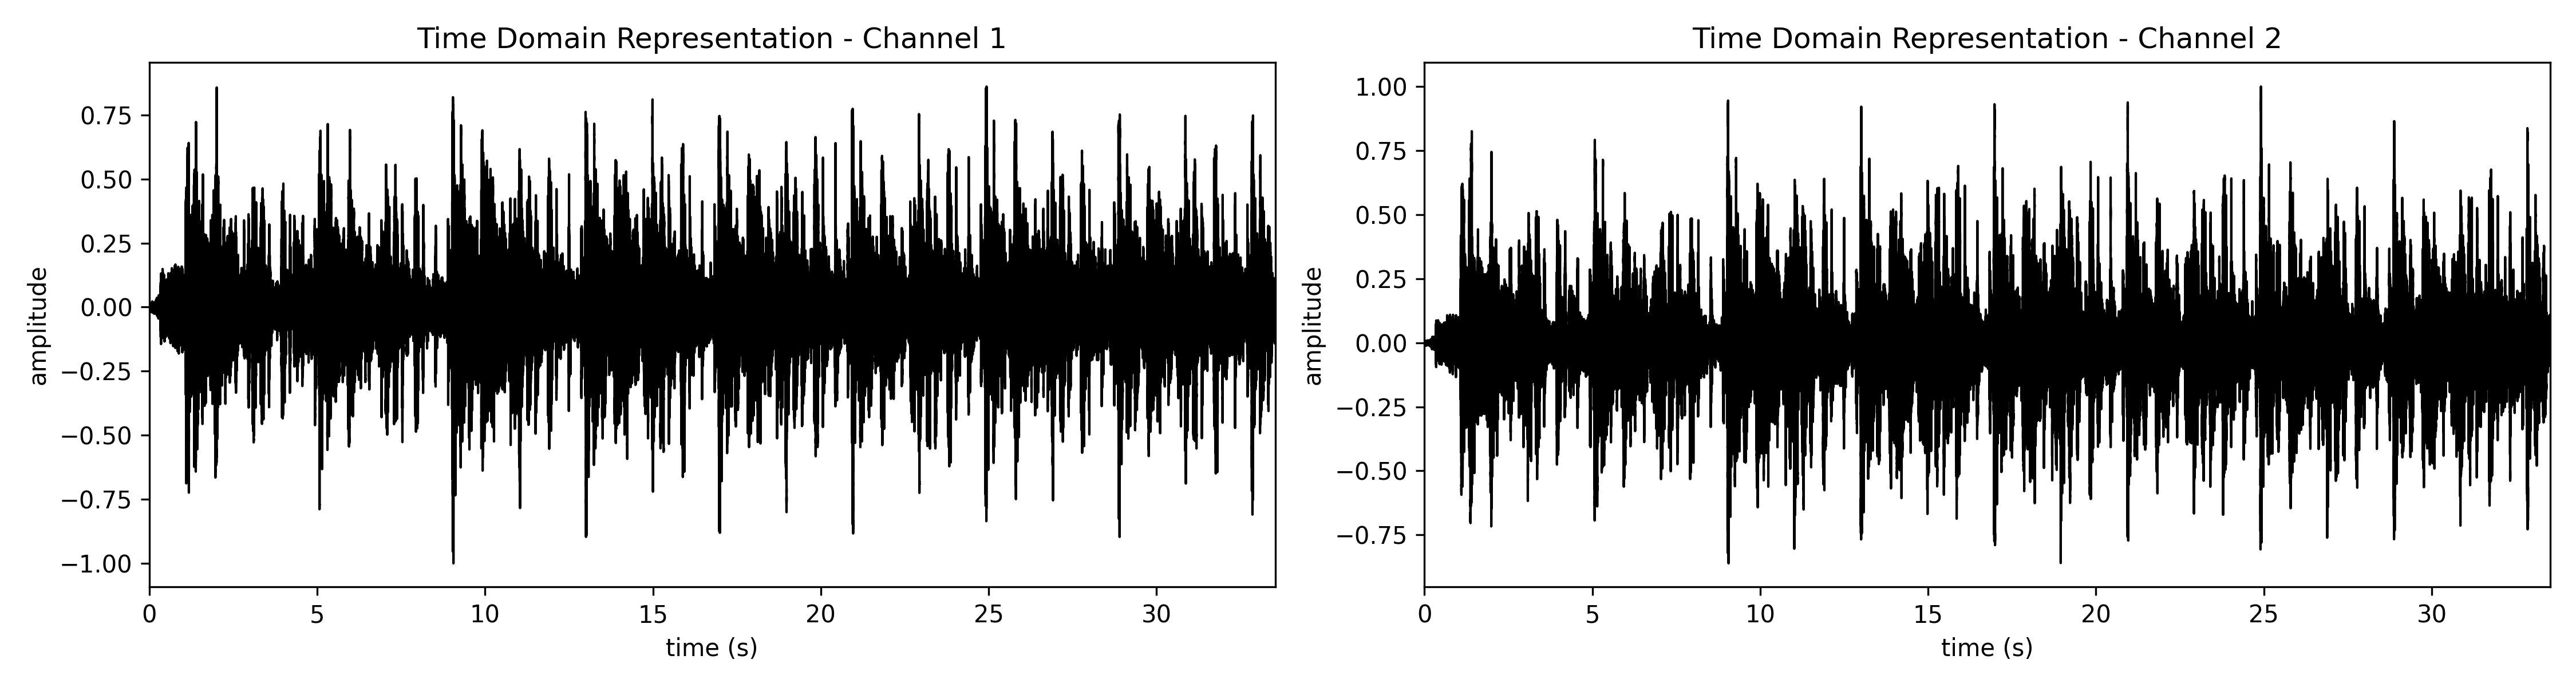
\includegraphics[width=\textwidth]{../Result/wav-time-domain-TX.png}
        \caption{Original}
        \label{fig:t-audio-cyclic-bsc-original}
    \end{subfigure}
    % \hfill
    \begin{subfigure}[b]{\textwidth}
        \centering
        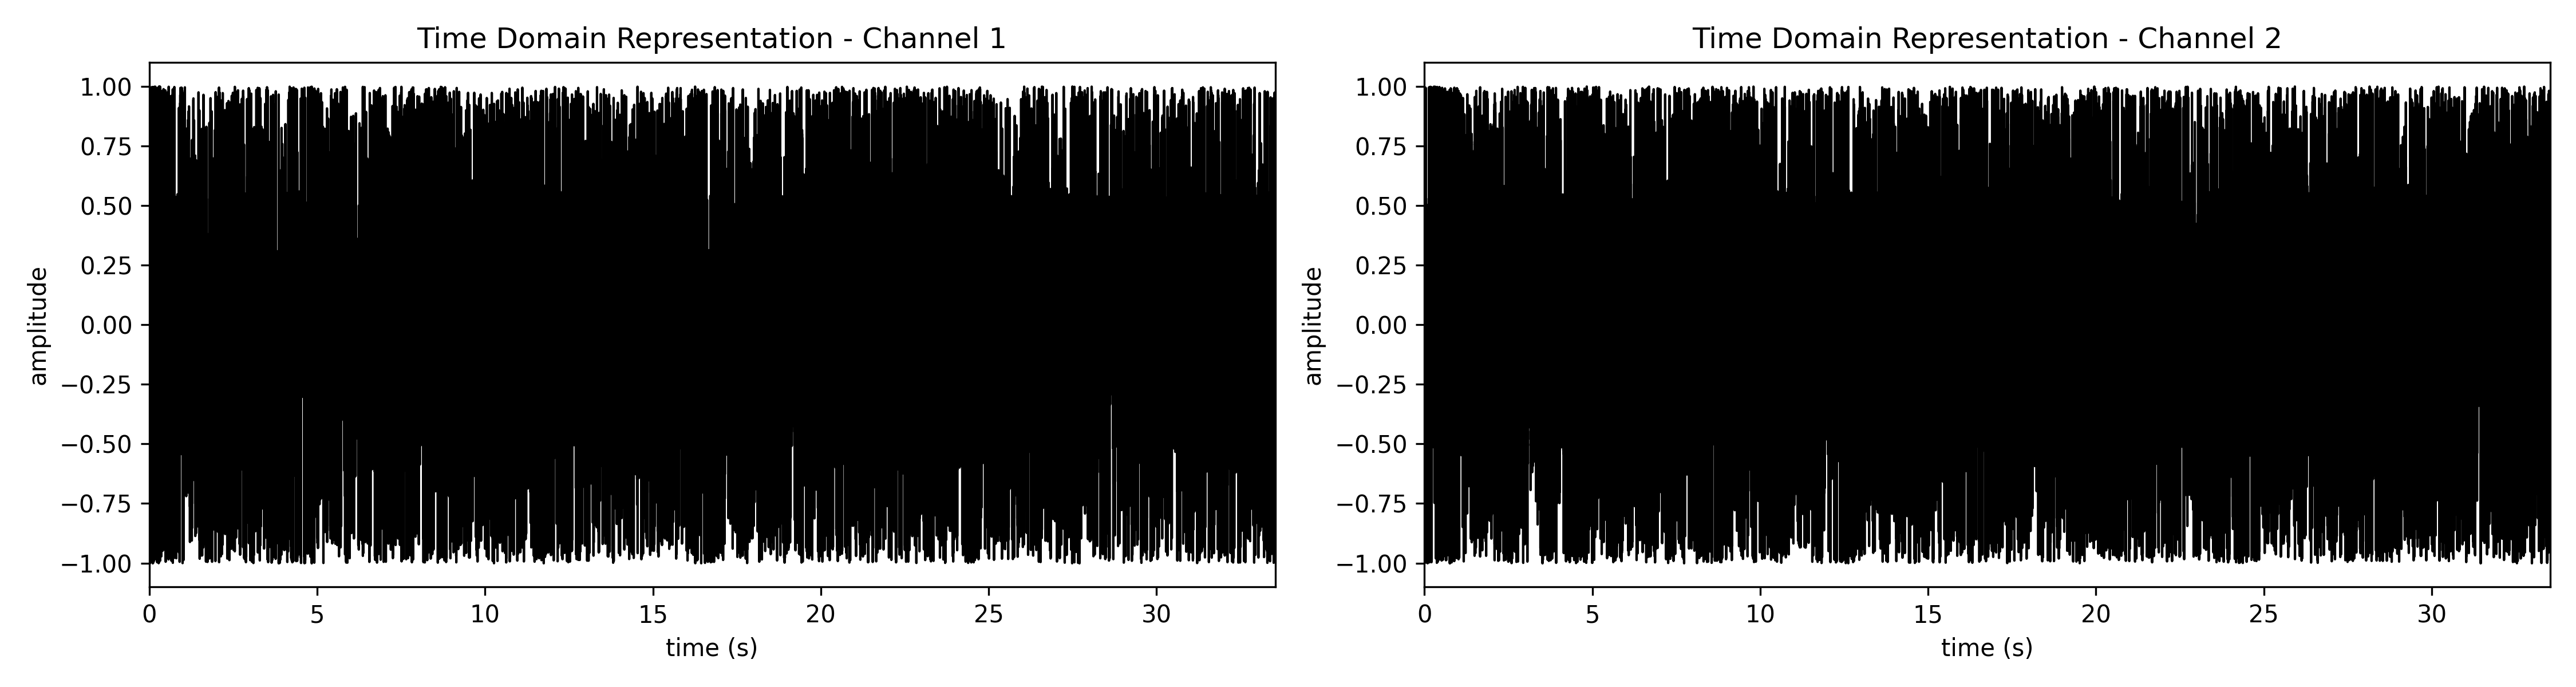
\includegraphics[width=\textwidth]{../Result/cyclic-bsc-wav-time-domain-RX.png}
        \caption{Without correction}
        \label{fig:t-audio-cyclic-bsc-no-correction}
    \end{subfigure}
    % \hfill
    \begin{subfigure}[b]{\textwidth}
        \centering
        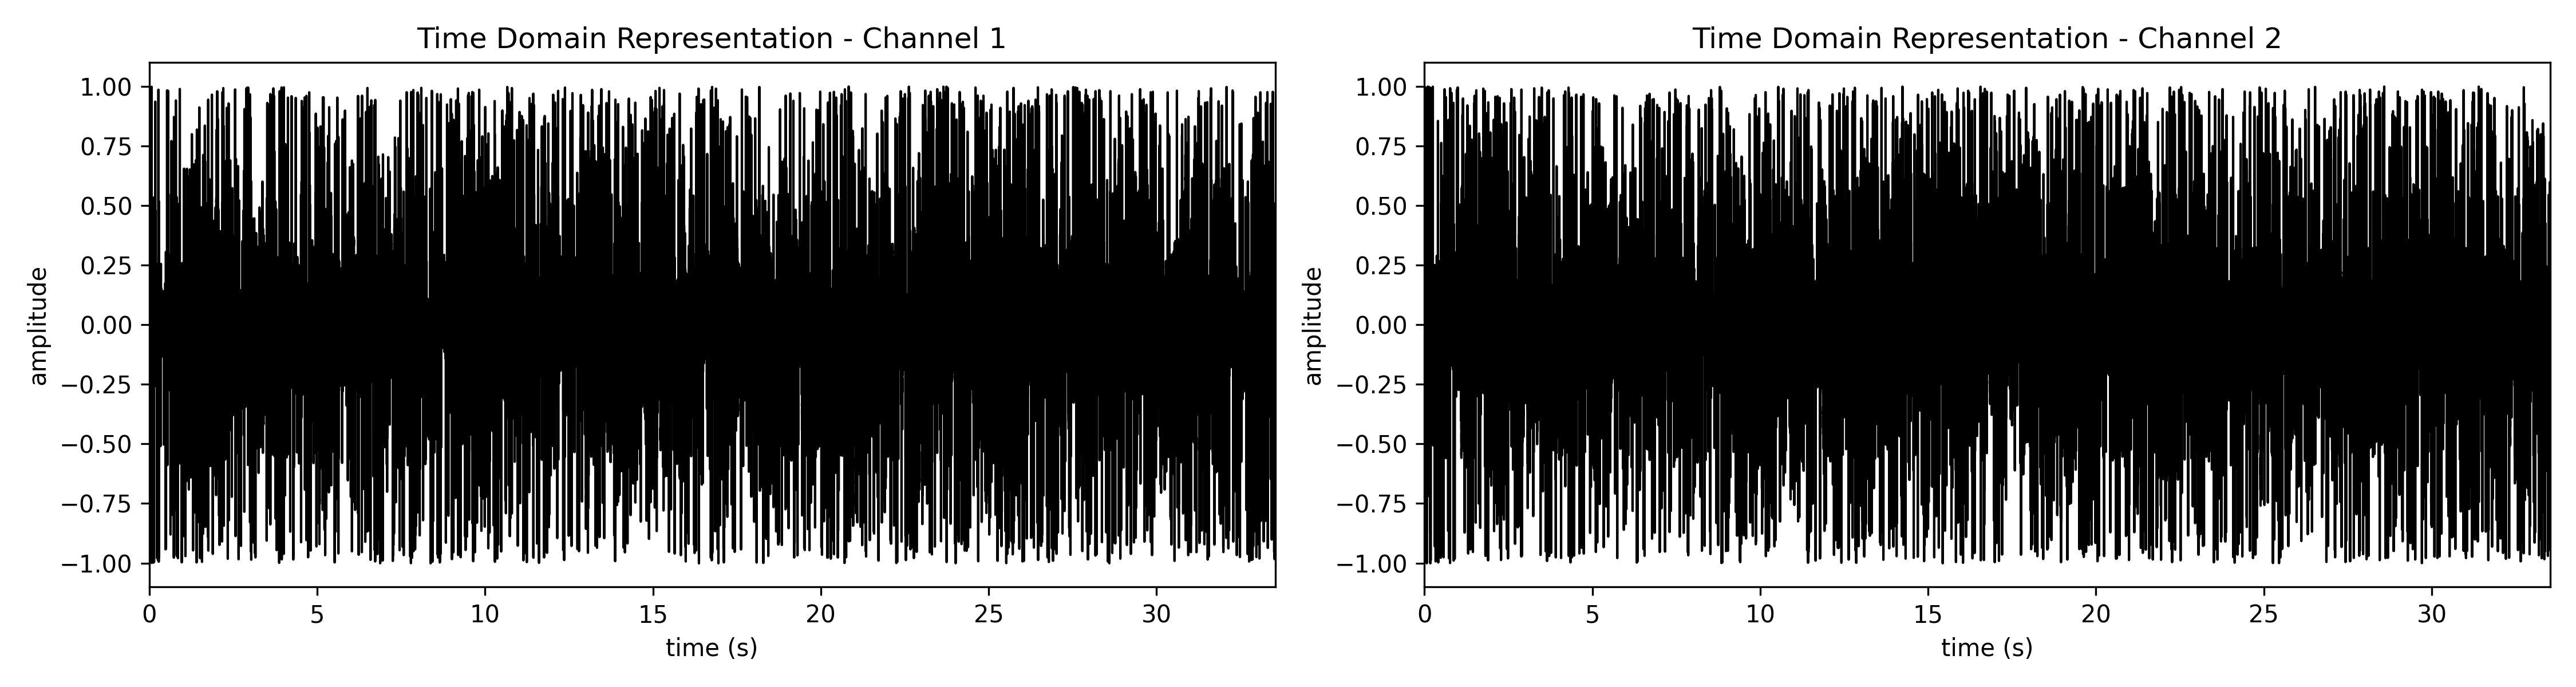
\includegraphics[width=\textwidth]{../Result/cyclic-bsc-wav-time-domain-RX-syndrome-corrected.png}
        \caption{Corrected}
        \label{fig:t-audio-cyclic-bsc-syndrome-syndrome-corrected}
    \end{subfigure}
       \caption{Audio encoded with Cyclic Hamming passed through BSC}
       \label{fig:t-audio-cyclic-bsc}
\end{figure}



\begin{figure}
    \centering
    \begin{subfigure}[b]{\textwidth}
        \centering
        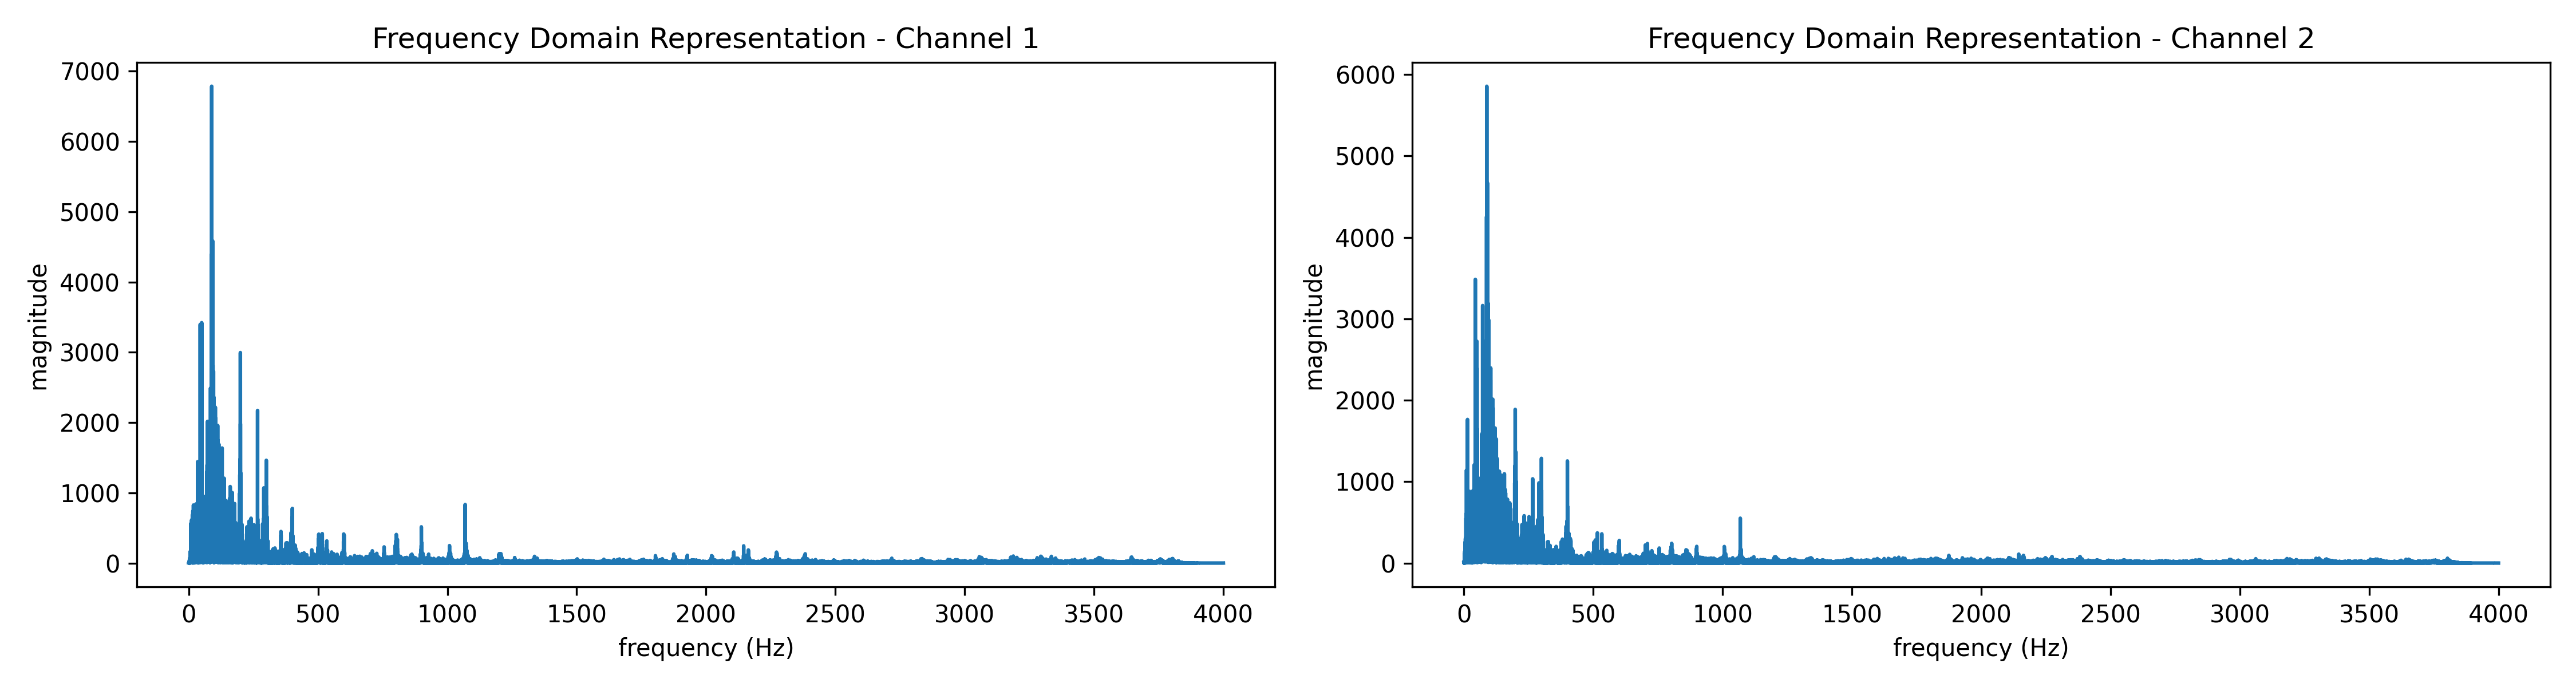
\includegraphics[width=\textwidth]{../Result/wav-frequency-domain-TX.png}
        \caption{Original}
        \label{fig:f-audio-cyclic-bsc-original}
    \end{subfigure}
    % \hfill
    \begin{subfigure}[b]{\textwidth}
        \centering
        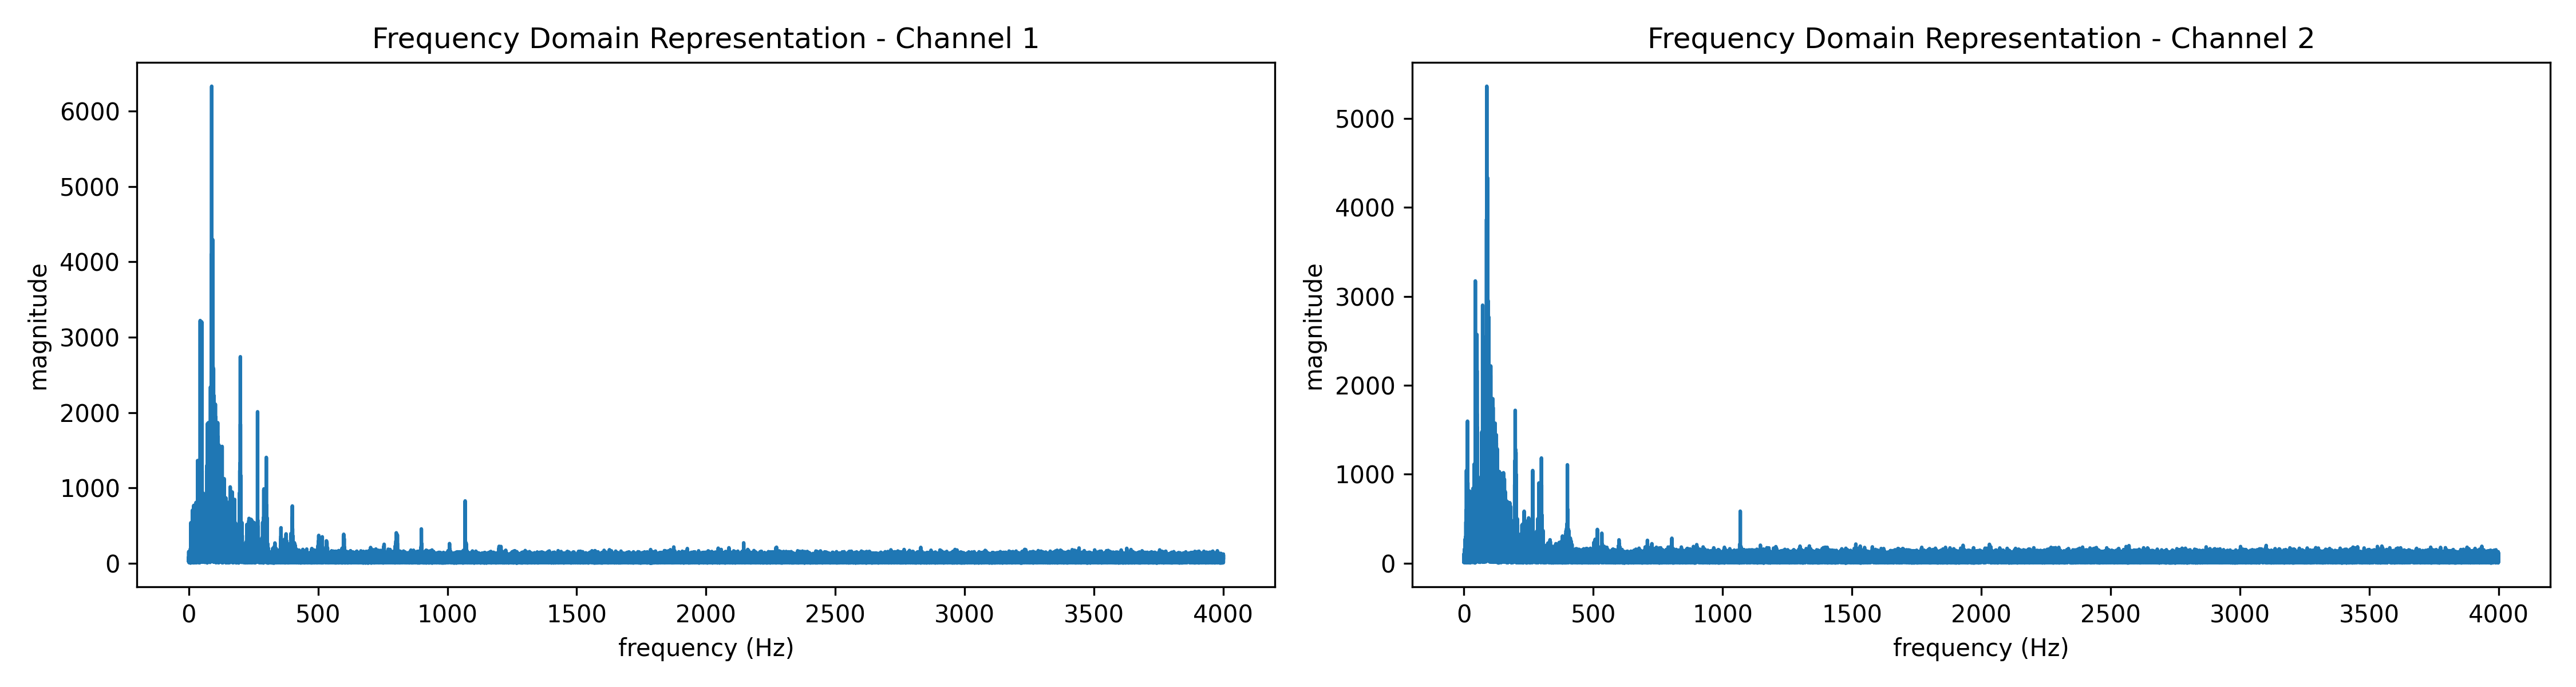
\includegraphics[width=\textwidth]{../Result/cyclic-bsc-wav-frequency-domain-RX.png}
        \caption{Without correction}
        \label{fig:f-audio-cyclic-bsc-no-correction}
    \end{subfigure}
    % \hfill
    \begin{subfigure}[b]{\textwidth}
        \centering
        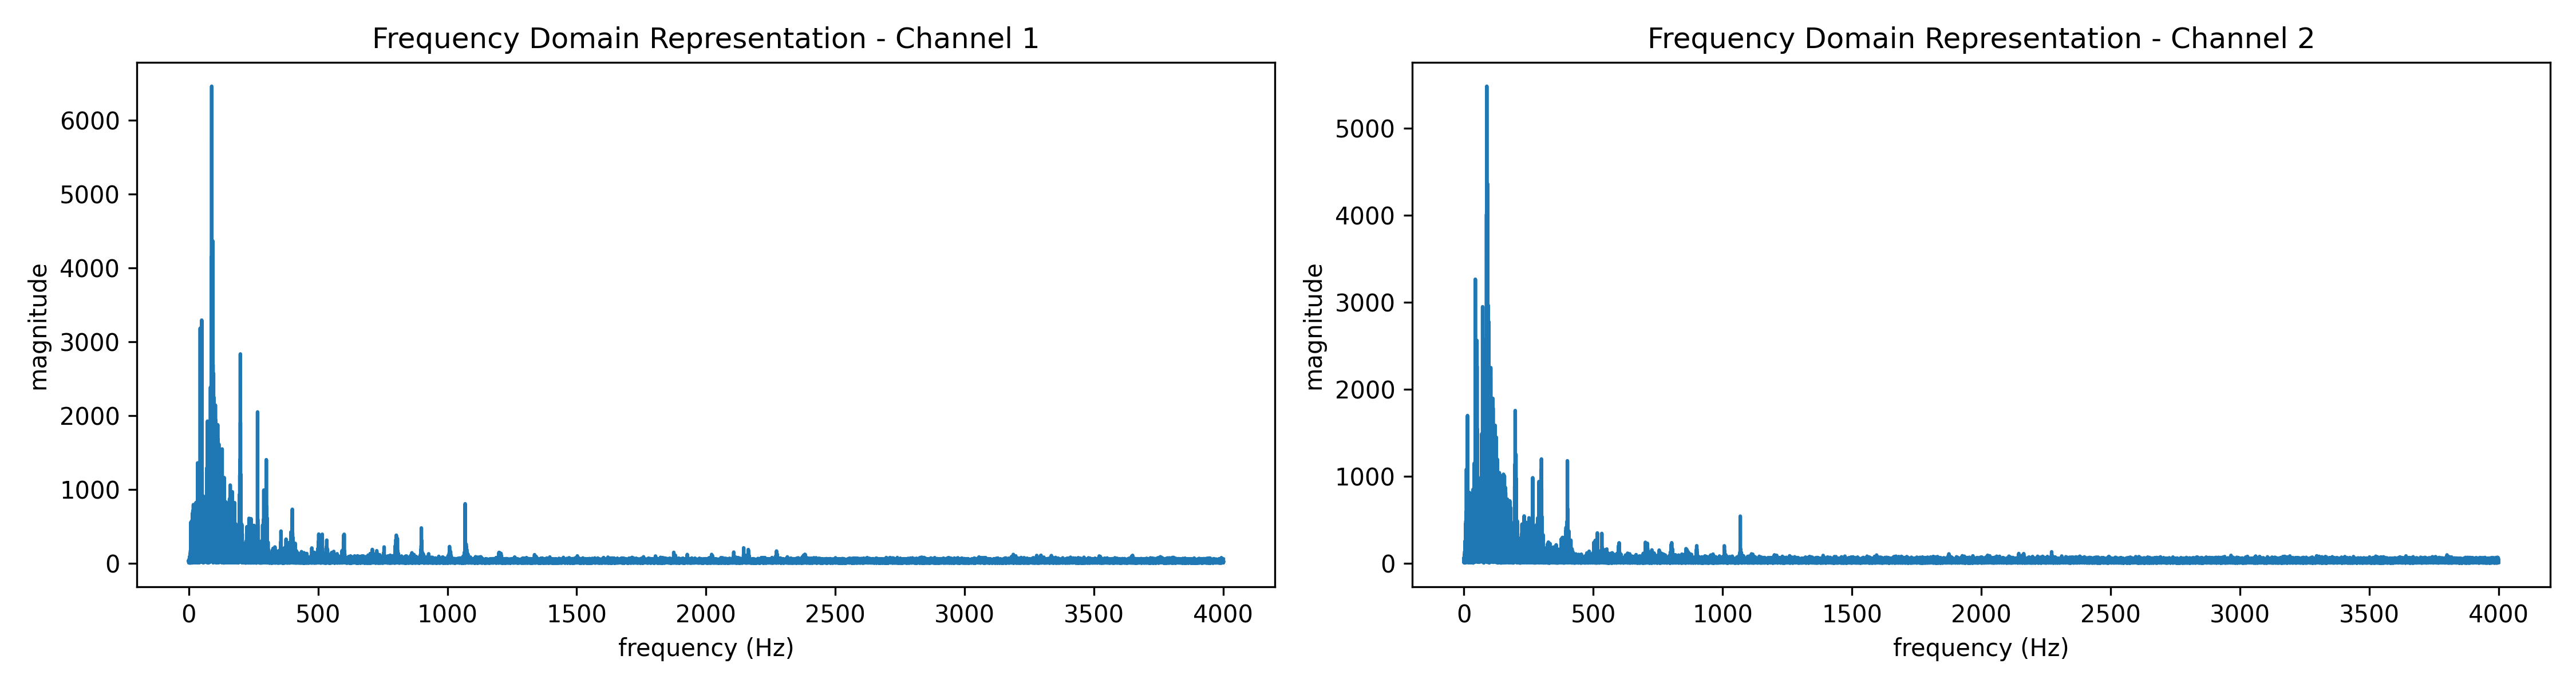
\includegraphics[width=\textwidth]{../Result/cyclic-bsc-wav-frequency-domain-RX-syndrome-corrected.png}
        \caption{Corrected}
        \label{fig:f-audio-cyclic-bsc-syndrome-corrected}
    \end{subfigure}
       \caption{Audio encoded with Cyclic Hamming passed through BSC}
       \label{fig:f-audio-cyclic-bsc}
\end{figure}






\subsection{LFSR Decoder}



\end{document}